% This is LLNCS.DEM the demonstration file of
% the LaTeX macro package from Springer-Verlag
% for Lecture Notes in Computer Science, 
% version 2.4 for LaTeX2e as of 16. April 2010
%
\documentclass[12pt]{llncs} %%%%%%%%%%%%%%%%%%%%% Used for
% drafting %%%%%%%%%%%%%%%%%%%%% 
%\documentclass{llncs}
%

\usepackage[colorlinks, linkcolor = black, citecolor = black, filecolor = black, urlcolor = blue]{hyperref} 

% APA Cite Package and initialization
%\RequirePackage{apacite}
\usepackage[apaciteclassic]{apacite} 
\bibliographystyle{apacite}

%
\usepackage{makeidx}  % allows for indexgeneration
%
\usepackage{color}
% 
\setcounter{tocdepth}{2}
% 
% make a proper TOC despite llncs
\makeatletter
\renewcommand*\l@author[2]{}
\renewcommand*\l@title[2]{}
\makeatletter 

\usepackage[latin1]{inputenc} 
\usepackage[T1]{fontenc} 
\usepackage[ngerman]{babel}

\usepackage{comment} 

\usepackage{tabularx} 
\usepackage{graphicx}


%\linespread{1.6} %%%%%%%%%%%%%%%%%%%%% Used for drafting %%%%%%%%%%%%%%%%%%%%%
\linespread{1.8} %%%%%%%%%%%%%%%%%%%%% Used for drafting %%%%%%%%%%%%%%%%%%%%%
\usepackage[margin=2.5cm]{geometry} %%%%%%%%%%%%%%%%%%%%% Used for drafting
% %%%%%%%%%%%%%%%%%%%%%

%=====================================================================================

\begin{document} 
%
\frontmatter          % for the preliminaries 
%
\pagestyle{headings}  % switches on printing of running heads
% \addtocmark{Hamiltonian Mechanics} % additional mark in the TOC
% 

\author{Gruppe 9\\
Lucas Garzarolli, 0955824,\\ 
David Eigenstuhler, 1257180,\\
Paul W�rtl, 0857021,\\
Gerald Zauner, 0756323\\}
\title{Medical Device Security}
\titlerunning{Medical Device Security}  % abbreviated title (for running head)
%                                     also used for the TOC unless
%                                     \toctitle is used
%\subtitle{Proposal}
\institute{Institut f�r Wirtschaftsinformatik\\
Software Engineering\\ 
Johannes Kepler Universitat Linz}
\maketitle
\vspace{2cm}
\begin{center}
Service Engineering SE (259.039 / WS 2014)\\
\vspace{0.3cm}
LVA Leiter: a. Univ.-Prof. Dr.Johannes Sametinger\\
\vspace{0.3cm}
18.12.2014 \\
\end{center}  


%=====================================================================================

%\newpage

\begin{comment}
\vspace{1cm}
\begin{abstract}
Here goes the abstract!\\
\vspace{1cm}
 
\textbf{Keywords: }
\textit{Keyword1, keyword2, keyword3}
\end{abstract}
\end{comment}

%=====================================================================================
%
\tableofcontents
%
\mainmatter              % start of the contributions
%
\title{Title?}
%
%=====================================================================================

 
\section{Einleitung}

Heutzutage sind Wireless Sensor Networks (WSNs) allgegenw�rtig und werden in
einer Vielzahl von Anwendungsgebieten eingesetzt. Im letzten Jahrzehnt fand
diese Technologie auch weitgehende Verbreitung im Bereich medizinischer
Diagnosesysteme. Medizintechnische Ger�te, die verwendet werden um WSNs
einzurichten k�nnen prinzipiell in implantierbare und externe Ger�te unterteilt
werden. Wobei Erstere dazu genutzt werden um spezifische Messungen im K�rper des
Patienten durchzuf�hren und somit dessen Gesundheit zu �berwachen. Diese Daten
werden an externe Ger�te �bermittelt, welche diese Informationen sammeln,
verarbeiten und gegebenenfalls Ma�nahmen einleiten um auf gesundheitskritische
Ereignisse zu reagieren. \cite{daniluk2012energy}

Auf Grund der zunehmenden Verbreitung von WSNs im medizinischen Bereich 
konzentriert sich auch die Forschung  verst�rkt auf die Entwicklung von sicheren
und stabilen Netzwerksystemen f�r medizinische Diagnosezwecke. H�ufig
eingesetzte implantierbare medizintechnische Ger�te  (IMGs), wie zum Beispiel
Herzschrittmacher, Blutzuckermessger�te und damit verbundene Insulinpumpen
k�nnen eine Art Sensornetzwerk in unserem K�rper bilden, welches im Vergleich zu
anderen WSNs von spezifischen Einschr�nkungen betroffen ist. Daher m�ssen bei
der Entwicklung von IMGs bestimmte Aspekte bez�glich der Stabilit�t, Sicherheit
und  der Energieressourcen  beachtet werden. \cite{grimes2004medical}

F�r die Entwicklung eines stabilen und sicheren Systems gilt es die Architektur
mit spezifischen L�sungen zu erweitern, um die Kommunikationskan�le abzusichern
und das System vor der Abh�rung, Einbringung oder Modifikation der zu
�bermittelnden Daten zu bewahren. In den folgenden Kapiteln werden wir auf
sicherheitsrelevante Aspekte, im Kontext der speziellen Merkmale von IMGs,
eingehen und die damit verbundenen Herausforderung an das System,
beziehungsweise dessen Entwurf, diskutieren.

\section{Effiziente Ressourcennutzung und Sicherheit}
Implantierbare medizintechnischen Ger�te (IMGs) erm�glichen Patienten sich frei
zu bewegen und ihren Alltag mit m�glichst geringen Einschr�nkungen zu
beschreiten, w�hrend die M�glichkeit besteht ihren Gesundheitsstatus
kontinuierlich zu �berwachen. \cite{hosseini2011lightweight}

IMGs k�nnen basierend auf deren Energieversorgung prinzipiell in zwei Gruppen
unterteilt werden:
\begin{itemize}
  \item Ger�te mit integrierten, nicht wiederaufladbaren Batterien (z.B.: Herzschrittmacher)
  \item Ger�te die induktiv betrieben werden (z.B.: Cochleaimplantat)
\end{itemize}

Wobei die meisten IMGs prinzipiell aus Sensoren und, Funkverbindungs-Modulen
bestehen, welche mittels einer Batterie mit Strom versorgt werden. Da die
Wartung dieser Ger�te  einen  chirurgischen Eingriffes erfordert und sich somit
sehr aufwendig gestaltet, gilt es die Energieeffizienz zu optimieren und die
Lebensdauer der Batterien zu maximieren. Dieser Aspekt sollte auch bei der
Entwicklung des Sicherheitskonzepts ber�cksichtigt werden, das die Grundlage f�r
eine zuverl�ssige und vertrauliche Daten�bertragung bildet und die Ger�te vor
unbefugten Zugriffen sch�tzt. Des Weiteren ist, auf Grund der kabellosen
�bertragung, ebenfalls die �bertragungsrate von IMGs eingeschr�nkt. Um die
Zeitfenster f�r potentielle St�rungen und Eingriffe zu minimieren, sowie Energie
zu sparen, sollte die �bertragung der Bits m�glichst schnell abgeschlossen und
somit auch die eingesetzte Hardware sorgf�ltig ausgew�hlt werden.
\cite{daniluk2012energy}


Die derzeitig verf�gbaren IMGs stellen diverse Funktionalit�ten zur Verf�gung,
wobei die Folgenden am verbreitesten sind:
\begin{itemize}
  \item das Monitoring bestimmter k�rperlicher Funktionen und Aktivit�ten,
  \item die Steuerung und direkte Programmierung, sowie indirekte Programmierung der IMGs �ber das Internet,
  \item die automatische oder gesteuerte Verabreichung von bestimmten Dosen eines Medikaments,
  \item sowie die M�glichkeit Informationen bez�glich der Implantate direkt vom
  Ger�t anzufordern \cite{daniluk2012energy}.
\end{itemize}

\subsection{Sichere und energieeffiziente  Netzwerkkommunikation}
Mit Sicherheitsaspekten auf der einen Seite und Energieeffizienz auf der anderen
Seite stehen sich zwei konkurrierende Ziele gegen�ber, wobei jedoch keines der
beiden vernachl�ssigbar ist - daher gilt es einen Kompromiss zu finden. Im
Folgenden werden theoretische Ans�tze diskutiert, deren Schwerpunkt auf der
Bereitstellung eines sicheren und energieeffizienten Netzwerks liegt.

Wie bereits erl�utert handelt es sich bei IMGs vereinfacht um Ger�te, die aus
Sensoren und Modulen zur Realisierung der Funkverbindung bestehen, die in den
menschlichen K�rper eingesetzt werden. Die Messwerte werden zu einer externen
Basisstation �bertragen, die sich am K�rper des Patienten, beziehungsweise an
dessen Kleidung, befindet. Die gesammelten Daten werden von der Basisstation an
ein mobiles Ger�t �bermittelt, welches die Rolle eines Brokers zwischen dem
Patient und dem behandelnden Arzt einnimmt. \cite{daniluk2012energy}

Ein m�glicher Ansatz ist die Entwicklung eines externen Sicherheitsger�ts,
welches gegebenenfalls auch in die Basisstation integriert werden k�nnte. Dieses
Ger�t w�re daf�r verantwortlich die Kommunikation zwischen den Sensoren und der
Basisstation zu �berwachen und auff�lliges Verhalten im Sensorennetzwerk zu
identifizieren, mit dem Ziel unzul�ssige Kommunikation zu unterbinden und somit
Angriffe weitgehend abzublocken. Verhalten kann mittels im Vorhinein definierter
oder dynamisch erlernter Regeln �berpr�ft werden. Durch das Blockieren
unzul�ssiger �bertragungen wird es erm�glicht die Batterie des IMGs zus�tzlich
zu entlasten und somit deren Lebensdauer zu erh�hen. \cite{daniluk2012energy}

Au�erdem w�re es sinnvoll einen Mechanismus zur Aggregation von Messdaten
anzuwenden, wodurch redundante Information eliminiert und  Energieressourcen
eingespart werden k�nnten. Um die Aggregation sicher gestalten zu k�nnen sind
eine Authentifizierung, sowie die Vertraulichkeit und Integrit�t der Daten
obligatorisch, wobei wohl �berlegt werden muss wie diese zu implementieren ist
um effizient zu laufen.  Des Weiteren ist es m�glich durch die Reduktion der
Signalst�rke und somit der Reduktion der Funkreichweite, Angriffe auf das System
zus�tzlich zu erschweren, da potentielle Angreifer physisch n�her an das Ger�t
heran m�ssen um die IMGs ansprechen zu k�nnen. In Verbindung mit einer
optimierten Positionierung der Sensoren und des Senders kann der
Energieverbrauch weiter optimiert werden. Derzeit werden in Experimenten die
optimalen Konfigurationen ermittelt. \cite{daniluk2012energy}

\subsection{Ein energieeffizientes Sicherheitsprotokoll}
Solide und bew�hrte Sicherheitsmechanismen, wie die  asymmetrische
Verschl�sselung, k�nnen hohe Kosten hinsichtlich der Rechenzeit und des
Energiekonsums verursachen.  Somit stehen sich auf der einen Seite mit der
Verwendung kryptografischer Methoden zur Sicherung des �bertragungskanals und
auf der anderen Seite mit der Langlebigkeit, sowie der Performance des IMGs
konkurrierende Ziele gegen�ber. Folgend wird ein Sicherheitsprotokoll
pr�sentiert, dass einerseits energieeffizient ist und andererseits einen
angemessenen Grad an Sicherheit bietet.

F�r das Sicherheitsprotokoll werden folgende Ziele definiert:
\begin{itemize}
  \item Vetraulichkeit: unbefugte Dritte k�nnen gesendete Nachrichten nicht lesen,
  \item Autorisierung: Nachrichten von unautorisierten Dritten werden erkannt und abgewiesen,
  \item Integrit�t: Nachrichten k�nnen nicht von Dritten manipuliert werden,
  \item sowie keine Wiederholbarkeit: ordnungsgem��e Nachrichten k�nnen nicht
  von Dritten unrechtm��ig repliziert und erneut gesendet werden \cite{hosseini2011lightweight}.
\end{itemize}

Im Folgenden wird erl�utert, wie diese Ziele effizient und ressourcensparend
erreicht werden, zuerst wird auf Vorraussetzungen eingegangen und dann das
Grundprinzip des Protokolls erl�utert. Eine leicht zu implementierende
Alternative zur asymmetrischen Verschl�sselung ist die symmetrische
Kryptographie, da in jedem Fall ein physischer Kontakt zwischen dem Patienten
und dem behandelnden Arzt stattfindet, stellt auch die vertrauliche, physische
�bergabe eines Schl�ssels kein Problem dar. Das hier vorgestellte Konzept sieht
eine ebensolche symmetrische Verschl�sselung zwischen dem IMG und der
Basisstation, zu der die Messdaten �bertragen werden, vor. Der symmetrische
Schl�ssel wird hierbei auf dem implantierten Ger�t gespeichert und vertraulich
zur Konfiguration der Basisstation an den behandelnden Arzt und den Patienten
weitergegeben. \cite{hosseini2011lightweight}

Eine Schl�ssell�nge von 80 Bit und Datenblock-Gr��e von 64 Bit sind speziell an
die Anforderungen von IMGs angepasst. Zur Entschl�sselung wird ein 64 Bit
ultra-lightweight Block Cipher Decryptor verwendet. Weiters verf�gt jedes
implantierte Ger�t �ber eine abgespeicherte 32 Bit lange Seriennummer, die unter
allen IMGs, die das gleiche Protokoll verwenden, eindeutig ist. Das IMG und die
Basisstation haben einen Z�hler der mit 0 initialisiert wird und ebenfalls eine
L�ge von 32 Bit hat, bei jeder gesendeten Nachricht wird er um eins erh�ht -
wodurch Nachrichten von unbefugten Dritten nicht repliziert werden k�nnen. \cite{hosseini2011lightweight}

Das Grundprinzip des Protokolls ist simpel gehalten. Anstatt einer gew�hnlichen
Authentifizierung werden zwei Z�hler verwendet, einer im IMG und einer in der
Basisstation. Bei jedem Sendevorgang wird der Z�hler der Basisstation erh�ht,
wenn der Z�hler der Basisstation h�her ist, als jener des implantierten Ger�ts
wird die Nachricht angenommen und der Z�hler der des IMGs auf den Wert des
anderen Z�hlers gesetzt, somit kann ausgeschlossen werden, dass Nachrichten
wiederholt werden. Durch die Verschl�sselung der Nachrichten kann das Auslesen
des Z�hlers, beziehungsweise die Manipulation der Nachricht, ausgeschlossen
werden. Au�erdem wird durch diese Methode gew�hrleistet, das das System nicht
neu synchronisiert werden muss, wenn eine Nachricht verloren geht. Da das
implantierte Ger�t lediglich einen Z�hler und einen Vergleichsmethode ben�tigt,
wird nur sehr wenig Rechenleistung in Anspruch genommen. Um die Sicherheit zu
erh�hen ist es optional m�glich den Z�hler jeweils um eine kleine Zufallszahl zu
erh�hen. \cite{hosseini2011lightweight}

Das Protokoll ist so ausgelegt, dass so wenig Hardware Module als m�glich
verwendet werden. Durch den Einsatz eines ultra-lightweight Block Cipher, wie
zum Beispiel PRESENT-80, kann der Einsatz eines energie-ineffizienten
Random-Access Memories vermieden werden um die beschriebenen Operationen
durchzuf�hren. \cite{hosseini2011lightweight}

Basierend auf der minimalistisch gehaltenen Logik und den sorgf�ltig
ausgew�hlten Hardware Komponenten, wird ein Protokoll geboten, welches im
Hinblick sowohl auf die Sicherheitskomponente als auch bez�glich der
Energieeffizienz als ausreichend angesehen werden kann.

\section{Allgemeine und spezielle Sicherheitsziele}

Die Themen Sicherheit und Risiko r�cken immer dann in den Mittelpunkt des
�ffentlichen Interesses, wenn durch Fehler in Ger�ten oder technischen Systemen
Menschen zu Schaden gekommen sind. Gefahren und Unf�lle k�nnen durch
menschliches Versagen ausgel�st werden, aber auch durch technische Defekte in
Systemen unterschiedlichster Art. Systeme die nicht vor Missbrauch gesch�tzt
werden oder auch andere sicherheitstechnischen Schw�chen aufzeigen, sind nicht
sicher und stellen ein erh�htes Risiko f�r Personen dar. [L�w, Pabst & Petry
2010, S. 9] 

Benutzer von technischen Ger�ten haben verst�ndlicherweise sehr hohe
Erwartungen an die Sicherheit von Systemen und die Reduzierung der Risiken und
Defekten. Hersteller wollen sichere Produkte kosteng�nstig entwickeln durch
Unf�lle vermeiden und die Kundenzufriedenheit erhalten. [L�w, Pabst & Petry
2010, S. 10] 

In den vergangenen Jahren ist der Der Anteil der
sicherheitsbezogenen, elektronischen Steuerungen und der Software in den
verschiedenen Produkten stark angestiegen. Daraus ergibt sich nat�rlich eine
wachsende Komplexit�t der Systeme und Anforderungen an die Sicherheit der
Ger�te. In aktuellen Kraftfahrzeugen finden sich schon bis zu 80 verschiedene
elektronische Steuerger�te die f�r Sicherheit der Passagiere sorgen. Diese
Entwicklung spiegelt sich jedoch in fast allen Bereichen wieder, unteranderem
auch  bei Medizinger�ten. Im Bereich der Medizintechnik spielt das Thema
Sicherheit und Zuverl�ssigkeit eine sehr wichtige Rolle. Die Software in diesen
Chips, die zu einem sicheren Betrieb der Ger�te beitr�gt, muss dann jedoch
stabiler und zuverl�ssiger funktionieren als etwa das Betriebssystem eines
heutigen Laptops, das den Betrieb ab und zu durch einen Neustart unterbrich t,
wenn es meint, �berlastet zu sein. [L�w, Pabst & Petry 2010, S. 10] 

Um
Anforderungen an Sicherheiten von Produkten erf�llen zu k�nnen, ist die
Anwendung von Sicherheitsnormen dringend erforderlich. Diese Normen beschreiben
Standards, welche von der Mehrzahl der Fachleute als korrekt anerkannt wird und
sich auch in der Praxis gut bew�hrt hat. Die Anwendung der Regeln unterst�tzt
zus�tzlich die nachweisbare Erf�llung der Sicherheitsanforderungen an Produkte.
[L�w, Pabst & Petry 2010, S. 11]

\subsection{Normen f�r die Sicherheit von Medizinprodukten}

Einen Stand der Technik widerspiegelndes Dokument definiert sich als Norm. Eine
Norm regelt und erleichtert somit durch Festlegungen allgemeine und
wiederkehrende Anwendungen, wie zum Beispiel Herstellungsprozesse,
Pr�fverfahren, sowie Produkteigenschaften. Sie k�nnen sich somit sowohl auf
Gegenst�nde als auch auf Verfahren beziehen. [R�lleke 2010, S. 605] 

Normen haben
f�r sich genommen keinerlei Gesetzeskraft. Ihre Anwendung f�r Produkte,
Hersteller, Betreiber und Anwender ist somit freiwillig. Erst durch Rechtsakte
k�nnen Normen Verbindlichkeit erlangen, etwa wenn auf sie in privaten Vertr�gen
oder in Gesetzen und Verordnungen Bezug genommen wird. [R�lleke 2010, S. 606]

Nun wollen wir auf Normen in Bezug auf Medizinprodukte n�her eingehen. Ein
Medizinprodukt ist ein einzelnes oder mit anderen Medizinprodukten verbundenes
Instrument, Apparat oder Vorrichtung, welche einschlie�lich der f�r ein
einwandfreies funktionierendes Medizinproduktes eingesetzte Software, die vom
Hersteller zur Anwendung f�r Menschen mittels ihrer daf�r vorgesehenen
Funktionen benutzt wird. Die Einhaltung grundlegender Anforderungen bei
medizinischen Produkten ist nach der jeweiligen Europ�ischen Richtlinie zu
erf�llen. [R�lleke 2010, S. 606] 

F�r alle Medizinprodukte gilt die "`DIN EN ISO
14971"'. Da diese Norm, als Prozessstandard noch die gr��te Produktn�he
aufweist, wollen wir sie an dieser Stelle etwas n�her darauf eingehen. Die Norm "`DIN EN
ISO 14971"' wurde spezifisch f�r die Herstellung von Medizinprodukten entwickelt
und behandelt sich mit dem Erkennen, Bewerten und Minimieren von Risiken, die
nat�rlich in der erster Linie Patienten betreffen k�nnten. [R�lleke 2010, S.
607] Das Risiko l�sst sich, neben subjektiv gepr�gten Parametern, auch durch
folgende 2 Faktoren charakterisieren:\\
\begin{itemize}
  \item Wahrscheinlichkeit des Auftretens eines Schadens
  \item Auswirkung des Schadens
\end{itemize}

Die Risikomanagementnorm "`DIN EN ISO 14971"' kann ebenfalls Prozesse zur
Identifizierung und Minimierung von Gef�hrdungen festlegen, die von Medizinprodukten ausgehen k�nnen. Einen Risikobereich vertretbar konkretisieren ist pauschal jedoch nicht m�glich. [R�lleke 2010, S. 608]

Wie schon zuvor erw�hnt beschreibt die Norm "`DIN EN ISO 14971"' eine
Risikomanagementnorm bzw. ein Verfahren. Die Abbildung 1 zeigt den, die in der ISO 14971 festgelegten, Risikomanagementprozess. Es gibt 4 Schritte f�r das Risikomanagement, welche zu beachten sind. [Rau 2010, S. 129]
\begin{itemize}
  \item Risikoanalyse (risk analysis)
  \item Risikobewertung (risk evaluation)
  \item Risikokontrolle (risk control)
  \item Postproduktionsinformationen (post-production information)
\end{itemize}

\begin{figure}[hbt]
    \centering
    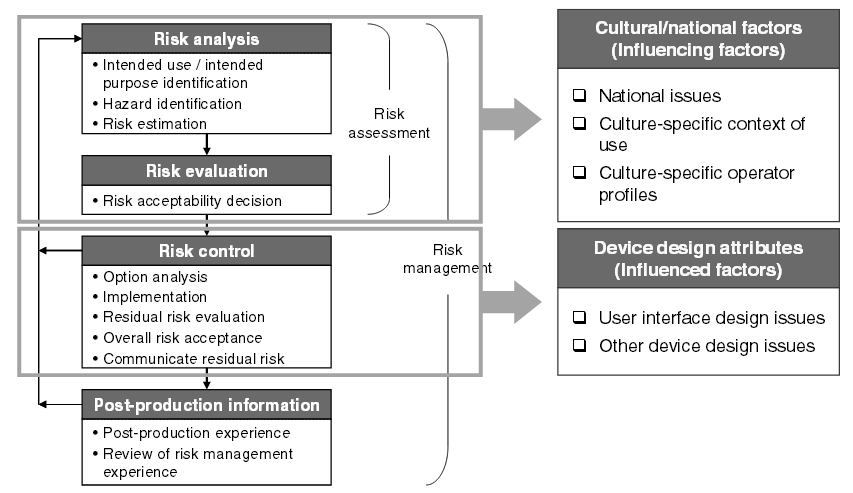
\includegraphics[width=1\textwidth]{resources/Definition_von_Informationssicherheit.png}
    \caption{Riskomanagement and Faktoren f�r kultur�bergreifende Gestaltung von Medizinprodukten [Rau 2010, S. 129]}
    \label{fig:risk_mgmt}
\end{figure}


\subsection{Definition von Informationssicherheit}

Der weiter verbreitete Begriff der IT-Sicherheit erf�llt nicht mehr die Anforderungen einer ganzheitlichen Betrachtungsweise, da Ger�te aus dem mobilen Bereich (wie in etwas Smartphones) nicht als IT-Systeme bzw. IT-Ger�te verstanden werden und dadurch oft �bersehen werden. Aus dieser Gegebenheit heraus, ist es normgerechter den Begriff Informationssicherheit zu verwenden. [Vogel, Gruetz 2010, S. 163]

Unter dem Begriff Informationssicherheit versteht man im Wesentlichen folgende
Punkte:
\begin{itemize}
  \item Vertraulichkeit\\
Die Informationen werden nur den dazu befugten Personen zug�nglich gemacht.
  \item Verf�gbarkeit\\
Die Informationen sind in angemessener Zeit aufrufbar.
  \item Integrit�t\\
Die Informationen bleiben richtig und vollst�ndig.
  \item Zurechenbarkeit\\
Die �nderungen der Informationen kann dem Urheber der �nderungen zugerechnet werden.
  \item Authentizit�t\\
Der Systembenutzer oder das System selbst ist tats�chlich derjenige bzw. dasjenige f�r den er oder es sich ausgibt.
\end{itemize}

Informationssicherheit dient der Aufrechterhaltung des Gesch�ftsbetriebs. In
weiterer Folge werden dadurch auch die Gesch�ftsrisiken minimiert und die Rendite und Gesch�ftschancen maximiert. Informationssicherheit ist somit der Schutz von Informationen vor einer Vielzahl von unternehmerischen Bedrohungen. [Vogel, Gruetz 2010, S. 163]

Die Informationssicherheit unterst�tzt somit das Unternehmen und darf nicht als
Hindernis angesehene werden. Welche Sicherheitsziele nun gelten, also beispielsweise welches Ma� an Vertraulichkeit bzw. Verf�gbarkeit f�r die Informationen gelten soll, sollte jedes Krankenhaus verbindlich und hausweit g�ltig in den Sicherheitslinien festlegen. Folgende Ziele k�nnten in die Sicherheitslinien festzuschreiben sein:
\begin{itemize}
  \item Unternehmenswichtige IT-Systeme sind hoch verf�gbar
  \item Alle Systeme werden von einem Zugriff durch Unbefugte gesch�tzt
  \item Die Anforderungen an die �rztliche Schweigepflicht werden eingehalten
  \item Kosten f�r die Gesch�ftsprozesse werden optimiert
  \item Schadensf�lle durch nicht gesicherte IT-Systeme werden unterbunden
\end{itemize}
[Vogel, Gruetz 2010, S. 163]


\section{Angriffsarten und Angriffspfade}

Immer mehr klassische Medizinger�te werden durch neuere innovative Ger�te ersetzt, deren Funktionalit�t durch Software gesteuert wird und die zum Austausch von Daten �ber das LAN (Local Area Network) oder WLAN (Wireless Local Area Network) kommunizieren. Diese Ger�te wachsen in die IT eines Krankenhauses hinein und unterliegen somit auch deren Gefahrenpotential. In den letzten Jahrzehnten waren in fast allen H�usern die Bereiche IT und Medizintechnik klassisch getrennt. In den letzten Jahren werden doch immer �fters herk�mmliche PCs zur Steuerung bzw. Auswertung der Daten von Medizinger�te. Auch fordert das Krankenhauspersonal erfasste Daten m�glichst �berall im Haus verf�gbar zu haben. Hierbei wird oft auf eine gemeinsam genutzte LAN-Kabel-Infrastruktur zur�ckgegriffen. Dabei ergeben sich jedoch folglich einige Sicherheitsprobleme. [Vogel, Gruetz 2010, S. 162]

Die Medizintechnik, die bisher quasi, in einer sicheren Umgebung arbeiten
konnte, hatte bisher keinerlei b�sartige Ein- und Angriffe waren zu erwarten, da es sich meist um nicht vernetzte Ger�te handelte. Diese Ger�te waren zus�tzlich auch noch mit propriet�ren Betriebssystemen ausgestattet oder in abgeschlossenen Netze ohne Zugang zur Au�enwelt, geschweige denn zum Internet. Auf der anderen Seite haben wir die moderne IT, die seit Jahren mit Viren und Trojanern, mit Fehlern in Betriebssystemen und Software leben muss. Dadurch hat sich ein reichhaltiges Wissen zur Gefahrenabwehr angeh�uft. [Vogel, Gruetz 2010, S. 162]

\subsection{Sicherheitsangriffe}
Aus der Gegebenheit heraus, dass in Krankenh�user dieselben bis sehr �hnliche
IT-Infrastrukturen wie in anderen Unternehmen zum Einsatz kommen, ergeben dieselben  klassischen IT-Sicherheitsprobleme und Angriffsarten.
\begin{itemize}
  \item Routing Protocoll Injection\\
Hierbei wird unbefugt die Routingtabelle von Gatewaysystemen verf�lscht
  \item Denial-of-Service-Angriffe\\
DoS-Angriffe unterscheiden sich in einem Punkt von anderen Angriffsarten. Bei dieser Art des Angriffs will der Angreifer nicht Zugang zum Netzwerk, sondern der Angriff hat den Zweck das System so stark zu �berlasten, dass eine normale Nutzung nicht mehr m�glich ist.  \item Die Anforderungen an die �rztliche Schweigepflicht werden eingehalten
  \item IF-Spoofing Angriff\\
Hierbei wird unter Vort�uschung einer falschen IP-Adresse Aktionen gegen fremde Systeme gestartet. Durch die Identit�tsverschleierung ist es oftmals schwierig den Verursacher zeitnah zu identifizieren.
  \item Password Cracking Angriffe\\
Dies stellt wohl die gebr�uchlichste Form von Angriffe auf IT-Systeme dar. Es wird versucht Zug�nge auf dem Zielsystem und die zugeh�rigen Passw�rter zu ermitteln.
  \item Man-in-the-middle-Angriff\\
Dies ist eine Angriffsart bei der sich eine initialisierende Kommunikationsbeziehung, bei der sich der Angreifer logisch genau zwischen den Partner befindet. Es wird dem Angreifer somit m�glich sein, Daten mitzulesen und ggf. auch zu manipulieren. Die Sicherheit kann in diesem Zusammenhang erh�ht werden, wenn sich beide Partner einer starken Authentifizierung beim Verbindungsaufbau unterziehen m�ssen.
\end{itemize}
[Laszlo 2004, S. 14]

\section{Kategorien von Ger�ten und Scope}
Eine Vielzahl an implantierbaren medizinischen Ger�ten existiert bereits. Wurden
in dieser Branche des US Marktes 2010 bereits 32,3 Mrd Dollar umgesetzt, so ist
davon auszugehen das einerseits aufgrund einer demographischen andererseits
einer technischen Entwicklung dieser weiter am Wachsen ist.

Das WallStreet Journal beschreibt 2011 die elf h�ufigsten IMGs. \cite{wallstreet2011eleven}

\begin{figure}[htb]
    \centering
    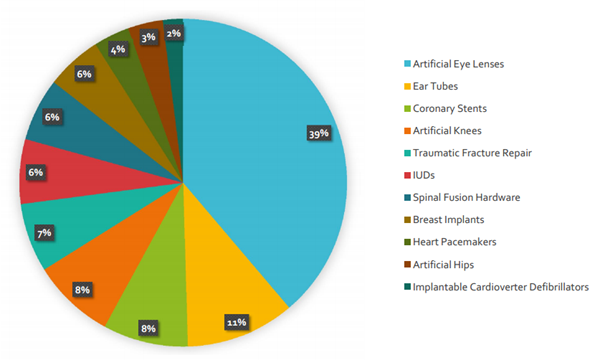
\includegraphics[width=1\textwidth]{resources/the_eleven_most_implanted_medical_devices_in_america_in_2011.png}
    \caption{The Eleven Most Implanted Medical Devices In America in 2011
    \protect\cite{wallstreet2011eleven}}
    \label{fig:11_most_med_dev}
\end{figure}

Einschr�nkend auf implantierbare Ger�te (IMG) sind Ger�tekategorien wie
Herzschrittmacher, Defibrilatoren, Insulinpumpen  und Neurostimulatoren in
dieser Arbeit von Bedeutung da diese drahtlose Kommunikation unterst�tzen.
\cite{gollakota2011they}

\section{Klassifizierung}

Bestehende Sicherheitsklassifikationen der Biomedizinischen Technik, der Medizin
oder der Informationssicherheit lassen sich nur teilweise auf die
Schutzklassifizierung von IMGs anwenden. Sie sind einzeln betrachtet zu
restriktiv um direkt zur Entwicklung von IMG Sicherheitsmodellen verwendbar zu sein.
\citeA{hansen2010taxonomy} entwickeln in ihrem Artikel durch das Verbinden
mehrerer Sicherheitsklassifikationen ein 'Big Picture' um sicherheitsrelevante
Verwundbarkeiten und infolge Gegenma�nahmen zu entwerfen. \cite{hansen2010taxonomy}

\subsection{Biomedizinische Technik}
Speziell in europ�ischen L�ndern m�ssen Hersteller von IMGs hohen Standards beim
Entwerfen und Testen ihrer medizinischer Produkten entsprechen.
Das 'National Research Ethics Service' in den UK klassifiziert folgende
schwerwiegende unerw�nschtes Ereignisse, welche auftreten k�nnen:
\begin{itemize}
  \item Resultiert in Tod
  \item Lebensbedrohend
  \item Resultiert in Krankenhausaufenthalt bzw. Verl�ngerung dessen
  \item Resultiert in Behinderung bzw. Einschr�nkung
  \item Ruft eine kongenitale Anomalie oder einen Geburtsfehler hervor
  \item Ist auf eine andere Art medizinisch signifikant negativ
\end{itemize}
\citeA{hansen2010taxonomy} verwenden diese Klassifizierung um die Effekte von
IMG Manipulation zu definieren.

\subsection{Medizin}
Die ICD-10 (International Statistical Classification of Deseases and Related
Health Problems) sehen vier Kategorien f�r Komplikationen von IMGs vor:
\begin{itemize}
  \item \textbf{T82:} Komplikationen von Herz und Gef�� Implantaten
  \item \textbf{T83:} Komplikationen von urogenitalen Implantaten
  \item \textbf{T84:} Komplikationen von internen orthop�dischen Implantaten
  \item \textbf{T85:} Komplikationen von innenliegenden Implantaten
\end{itemize}
\cite{hansen2010taxonomy}

\subsection{Informationssicherheit}
Relevante Klassifikationen im Feld der Informationssicherheit werden
grunds�tzlich in zwei Gruppen aufgeteilt: 
\begin{itemize}
  \item Bedrohungen des Systems
  \item Evaluierung der Verwundbarkeit
\end{itemize}
\citeA{hansen2010taxonomy} lehnen sich an diese an und entwickeln daraus ihre
Risikoklassifikation f�r IMGs beziehungsweise deren Verwendung.

\subsection{Klassifikation der
Auswirkungen}\label{sec:klassifikation_auswirkungen} Die Kombination der
medizinischen Klassifikationen der Komplikationen mit den schwerwiegenden unerw�nschten Ereignissen der biomedizinischen Technik lassen
\citeA{hansen2010taxonomy} zu zwei Kategorien kommen:
\begin{itemize}
  \item IMG Aktivit�t
  \item Schwerwiegende Effekte
\end{itemize}
Vergleiche Abbildung \ref{fig:potentielle_folgen_imgs} f�r eine tabellarische
Gegen�berstellung der beiden Kategorien.\\
\begin{figure}[htb]
    \centering
    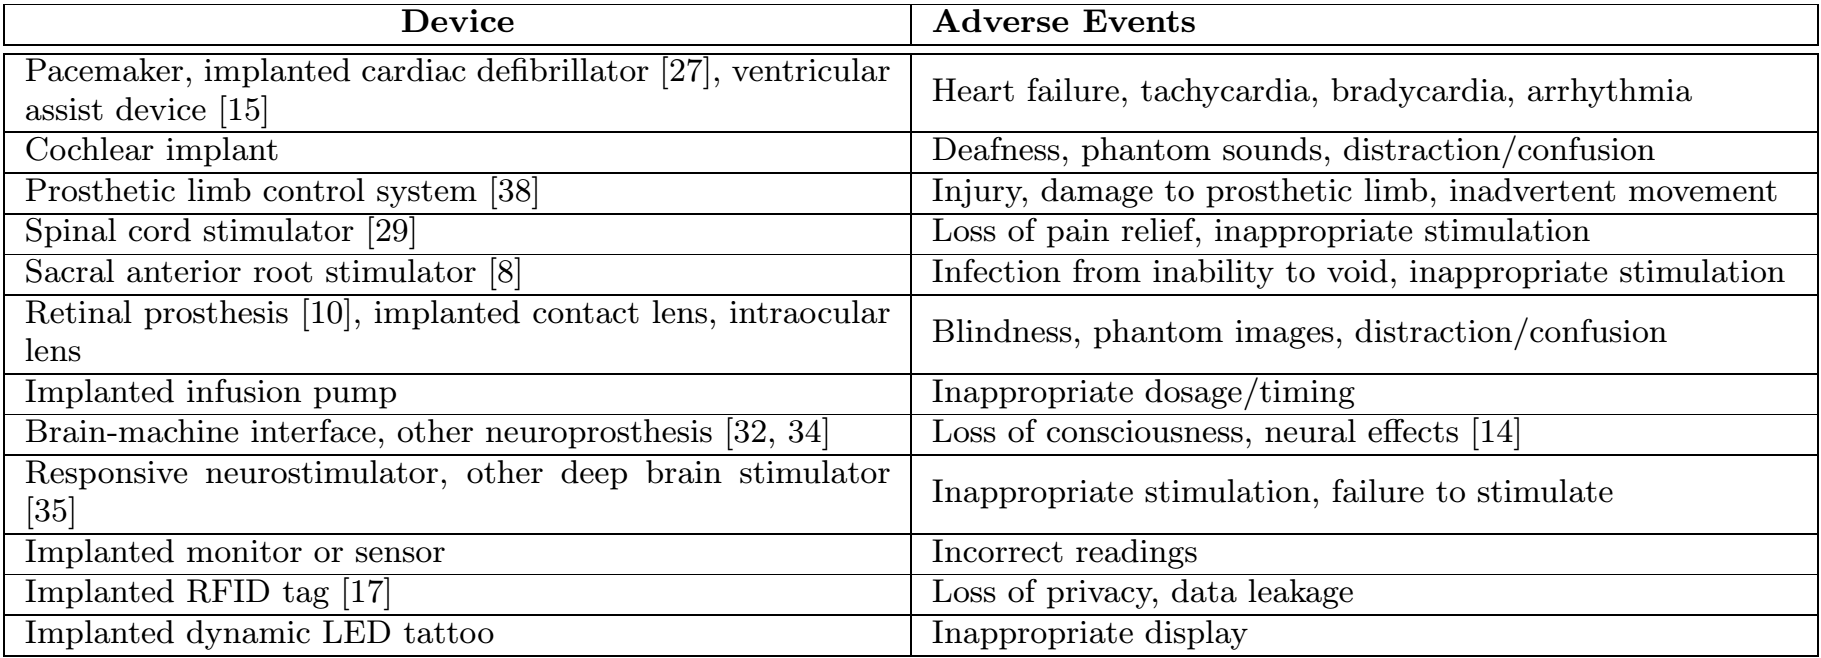
\includegraphics[width=1\textwidth]{resources/Potential_Adverse_Events_in_Various_Implantable_Medical_Devices.png}
    \caption{Potentielle schwerwiegende Folgen in IMGs
    \protect\cite{hansen2010taxonomy}}
    \label{fig:potentielle_folgen_imgs}
\end{figure}

\subsection{Klassifikation der Verwundbarkeit}
Die Vulnerabilit�t von IMGs h�ngt laut \citeA{hansen2010taxonomy} im
Wesentlichen von zwei verschiedenen Kategorien ab: Der N�he vom Angreifer zum zu
manipulierenden Ger�te und von der Funktion des Ger�tes an sich.

\subsubsection{Physische N�he: }
Zeitlich langanhaltender, direkter physischer Kontakt eines Angreifers zu
einem willigen oder bewusstlosen Patienten macht praktisch nahezu alle IMGs
offen f�r Angriffe. \citeA{hansen2010taxonomy} lassen in ihrer Arbeit jedoch diese
F�lle konkret aus, da sie sich auf vom Patienten unbemerkte Angriffe festlegen.
Sie definieren folgende physischen N�heverh�ltnisse zwischen Angreifer und
Patient:
\begin{itemize}
  \item Kontakt: Ber�hrung
  \item Kurz: bis zu 1 Meter
  \item Medium: 1 Meter bis 50 Meter
  \item Weit: �ber 50 Meter
  \item Sichtkontakt
  \item Netzwerk
\end{itemize}

\subsubsection{Funktion: }
Die Funktion des IMGs beeinflusst direkt sowohl die Vulnerabilit�t gegen�ber
unbefugte Ver�nderungen wie auch die Effekte welche daraus entstehen.
\citeA{hansen2010taxonomy} unterteilen in folgende vier Funktionsweisen von
IMGS:
\begin{itemize}
  \item Messend: Informationen vom Patienten oder seiner Umgebung sammeln
  \item Wirkend: Erwirkt einen Effekt, normalerweise therapeutischer Natur
  \item Informationsverabeitend: Aggregiert oder berechnet Informationen
  \item Kommunizierend: Kontakt mit anderen IMGs, externen Ger�ten oder dem
  Patienten
\end{itemize}

\subsection{Folgen}
Die schwerwiegenden Folgen, wie in Abschnitt
\ref{sec:klassifikation_auswirkungen} angesprochen werden von
\citeA{hansen2010taxonomy} anhand zweier Merkmale klassifiziert. Einerseits
welche Komponenten betroffen sind und andererseits die Dauerhaftigkeit der
Folgen.

\subsubsection{Betroffene Komponenten: }
Betroffen sein k�nnen neben dem manipulierten Ger�t ebenfalls in
Kommunikationskontakt stehende Ger�te sein. Diese k�nnen neben anderen IMGs
externe Ger�te wie Computer oder Anzeigen und Displays sein. Im schlimmsten Fall
betrifft es jedoch auch den Patienten selbst. Somit kann der Angriff direkte und
indirekte Auswirkungen hervorrufen. \cite{hansen2010taxonomy}

\subsubsection{Dauerhaftigkeit: }
Wenn der Effekt des Angriffs nach einiger Zeit wieder nachl�sst und
verschwindet oder nur solange anh�lt, solange der Angriff besteht sprechen
\citeA{hansen2010taxonomy} von einer tempor�ren Dauerhaftigkeit. Wird jedoch die
Software beziehungsweise die Firmware des IMGs ver�ndert sprechen die beiden
Autoren von einer persistenten Dauerhaftigkeit. Der schlimmste Fall, der
Tod des Patienten, f�llt ebenfalls in diese Kategorie.

\begin{figure}[htb]
    \centering
    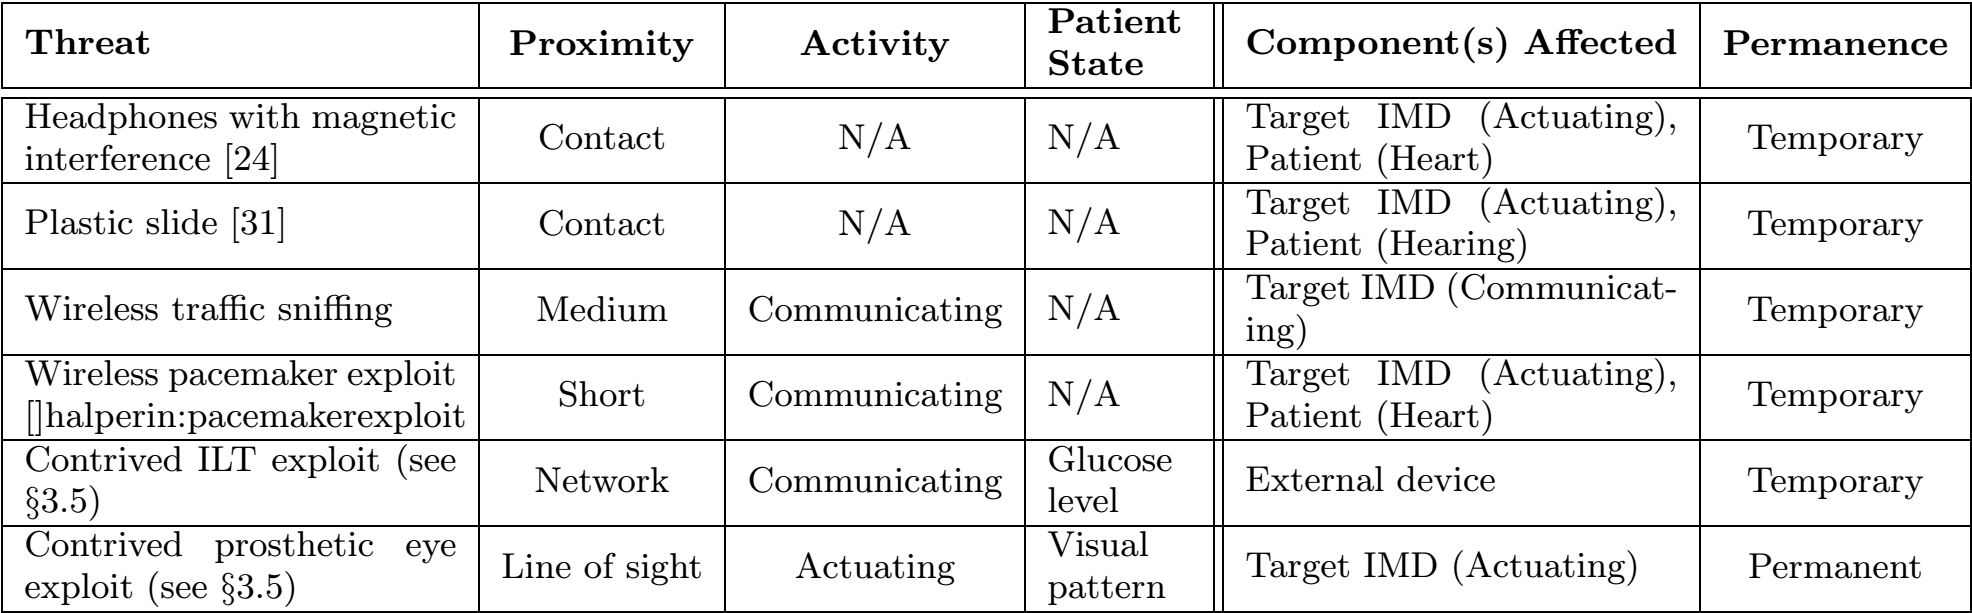
\includegraphics[width=1\textwidth]{resources/A_Breakdown_of_Several_Vulnerabilities_According_to_our_Classification.png}
    \caption{Eine �bersicht �ber mehrere Verwundbarkeiten anhand der
    Klassifikation von \protect\citeA{hansen2010taxonomy}}
    \label{fig:uebersicht_verwundbarkeiten}
\end{figure}

%%%%%%%%%%%%%%%%%%%%%%%%%%%%%%%%%%%%%%%%%%%%%%%%%%%%%%%%%%%%%%%%%%%%%%%%%%%%%%%%%%%%%%%%%%%%%%%%%%%%%%%%%%%%%%%%%%%%%%%%%%%%%%%%%%%

\section{Sicherheitsma�nahmen, Vorkehrungen und Verteidigungsstrategien}
Einerseits sind es vorbeugende Ma�nahmen welche Risiken verhindern oder zu
mindestens vermindern sollen und andererseits Ma�nahmen welche bei Angriffen
oder Schadenseintritt die damit einhergehenden Auswirkungen m�glichst gering halten.

\subsection{Pr�ventive Ma�nahmen}
Staatliche als auch supranationale Organisationen wie die Europ�ische Union
stellen grunds�tzliche Richtlinien f�r IMG's und den Umgang mit diesen zur
Verf�gung.

Hinsichtlich Medical Devices existiert von der FDA (Amerikanischen
Gesundheitsbeh�rde) einerseits ein Leitfaden f�r Medical Device Security
andererseits eine Erfahrungsdatenbank MAUDE (Manufacturer and User Facility
Device Experience Database) welche Usererfahrungen aufzeichnet �ber Medizinische
Ger�te hinsichtlich IT Sicherheitsrelevanter Belange. \cite{fda2014manufacturer}

Auf europ�ischer Seite existiert die Richtlinie 90/384/EWG des Rates vom 20.Juni
1990 zur Harmonisierung der Rechtsvorschriften f�r implantierbare medizinische
Ger�te. Die letztg�ltige �nderung beziehungsweise Berichtigung dieser Richtlinie
bezogen auf Anwendung beim Menschen ist aktuell in der Richtlinie 2007/47/EG
festgehalten. \cite{richtlinie2012eu}


Aktuell existieren mehrerer Frameworks durch welche einerseits bisherige Ziele
wie vern�nftige Brauchbarkeit und Betriebssicherheit  als auch Security und
Privacy bei IMG's erwirkt werden soll. \citeA{halperin2008pacemakers} stellt
ein derartige Framework vor mit welchem Sicherheit und Privatsph�re der Daten
zuk�nftiger IMG's evaluiert werden soll. Die Schwierigkeit besteht darin eine
Balance zwischen den genannten Ziele zu finden. Um Kommunikation mit IMG �ber
gr��ere Distanzen zu erm�glichen stellen \citeA{gollakota2011they} einen weiteren L�sungsansatz vor, welcher

\subsection{Aspekte der Betriebssicherheit und Anwendbarkeit}
Der Zugriff auf Daten muss durch berichtigte Ger�te gegeben sein da diese Daten
in normalen oder Notfallsituation sehr relevant sein k�nnen. Wie in Abbildung 2
am Beispiel eines Defibrilators dargestellt ergeben sich technische
Anforderungen an das Ger�t selbst, an die drahtlose Kommunikation und an
Ausfallsicherheit des gesamten Systems.

Um Betriebssicherheit und Anwendbarkeit zu erwirken sind nach \citeA{halperin2008pacemakers}
folgende Kriterien ausschlaggebend:
Der Zugriff auf Daten (Data access) muss f�r autorisierte Ger�te oder
Individuen bei Bedarf m�glich sein. Diesbez�glich sind jegliche Daten in
Verbindung mit einem IMG von Belangen.
Die gemessenen und gespeicherten Daten sollten ad�quat den Anforderungen an ein
System hinsichtlich ihrer Datengenauigkeit gen�gen. Dies kann auch f�r Zeitliche
Daten gelten.

Die Ger�te Identifikation ist wesentlich das beispielsweise bei einer Operation
ein Ger�t identifiziert werden muss und autorisierten Teilnehmern Rechte und
Informationen einger�umt sein m�ssen. Folglich gilt dies auch f�r eine
notwendige Konfigurierbarkeit und eine Updatebarkeit der Software. Sollten
Patienten mehrere IMG tragen oder mehrere IMG in Kommunikationreichweite
beispielsweise eines Programmer sein so ist es von N�ten das die Koordination
zwischen den Ger�ten gew�hrleistet ist. Dies ist auch unter dem Begriff
Multidevice coordination zusammengefasst. Um Sicherzustellen das jegliche Fehler
bei Ger�ten erkannt werden k�nnen sind Prinzipien der Auditierbarkeit
notwendigerweise zu ber�cksichtigen. Ressourceneffizienz ist wesentlich um eine
maximale Lebenszeit eines Ger�tes einerseit hinsichtlich des Auskommens mit
gespeicherter Energie andererseits bez�glich des maximalen
Verf�gbarkeitzeitraums selbst.

\subsection{Aspekte zu Ma�nahmen zur Erreichung  von Sicherheitszielen und Privatsph�re}
Nach \citeA{halperin2008pacemakers} sind folgende Kriterien hinsichtlich Ziele
der Sicherheit und Privatsph�re ausschlaggebend:\\
Autorisierung von Personal das nur bestimme Individuen ihnen zugestandene
Anwendungen durchf�hren k�nnen. Weiter verfeinert ist dies auch durch ein
Rollenkonzept werden indem Autorisierte Individuen Zugriff durch eine
zugewiesene Rolle erhalten. Unterschiedliche Rollen nehmen dabei beispielsweise
der Patient selbst, der Mediziner, der Ambulanz Computer oder der Ger�te
Hersteller ein.

\begin{figure}[htb]
    \centering
    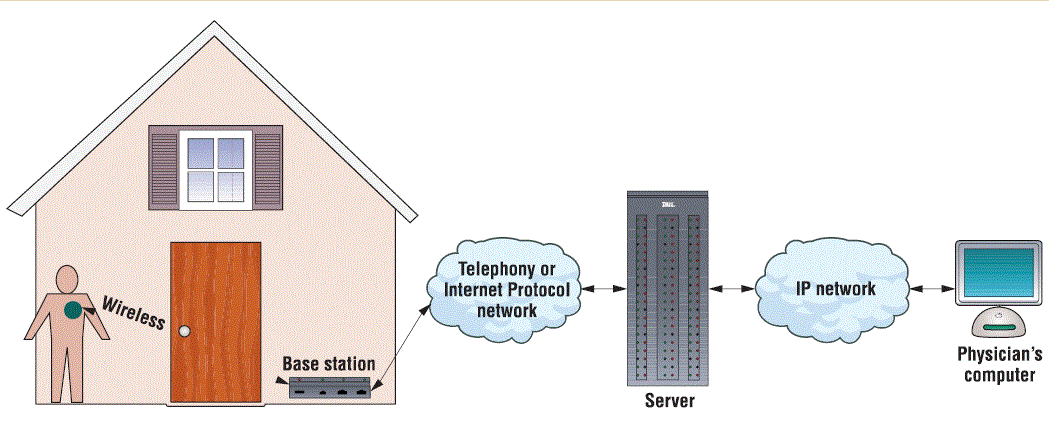
\includegraphics[width=1\textwidth]{resources/Beispiel_Defibrilator_und_home_monitoring.png}
    \caption{Defibrilator mit Home Monitoring durch Webzugriff}
    \label{fig:defibrilator_webzugriff}
\end{figure}

Kommuniziert ein Ger�t mit mehreren IMGs so muss sichergestellt werden das die
Kommunikation nur mit dem beabsichtigten Ger�t statt findet. Diese wird wiederum
durch Autorisierungs- und Authentifizierungsma�nahmen erreicht. Als
Zugriffsmodell k�nnte eine von \citeA{gupta2006criticality} vorgestellte L�sung
zum Einsatz kommen. Des weiteren stellt die Verf�gbarkeit einen (lebens-)
wichtigen Punkt dar, gerade wenn es Denial of Service Angriffe geht. Die
Ger�tesoftware muss ausreichend zuverl�ssig in Hinblick auf Implementierungs-
und Entwicklungsfehler sein. Ausreichende Abhilfe muss durch Softwaretests
seitens des Hersteller geschaffen werden. Ein fehlerhaftes Verhalten eines
Herzschrittmachers kann beispielsweise gravierende Auswirkungen f�r einen
Patienten haben.

Device existence privacy beschreibt dass das IMG nicht f�r andere
unautorisierte Ger�te sichtbar ist. Sollte trotzdem Sichtbarkeit gegeben sein
ist sicherzustellen das die Type des Ger�ts (Device type privacy) und die Ger�te
ID (Specific device ID privacy) nicht verraten werden, um einen m�glichen
Angriff zu unterbinden. Weiters sind Messdaten und Logs dieser unautorisierten
Personen vorzuenthalten. Es soll auch nicht m�glich sein, sollte das Ger�t
erkannt werden �ber einen Exploit den Tr�ger des Ger�tes zu identifizieren. Dies
wird als Bearer Privacy bezeichnet. Schlussendlich muss auch die Daten
Integrit�t jeglicher Daten welche mit dem Patienten und dem IMG in Verbindung
stehen gewahrt bleiben. Eine m�gliche Manipulation beispielsweise von Logdaten
k�nnte zu einem falschen Setting des Ger�tes f�hren und dies dem Tr�ger
schaden. \cite{halperin2008pacemakers}

\subsection{Aspekte der Kommunikation}
Ein Kommunikationskanal eines IMG's zu einem Personal Computer oder einem
Smartphone bringt zwar die Vorteile eines Datenaustausches mit sich, dadurch
entsteht jedoch auch ein m�glicher Angriffspfad. Abhilfe k�nnte dadurch
geschaffen werden das ein IMG unterschiedliche Schnittstellen f�r die
unterschiedlichen Ger�te mit welchen er kommuniziert anbietet. Dabei kann die
Art der Verbindung ob bidirektional oder unidirektional (nur senden oder nur
empfangen) einen entscheidenden Beitrag zur Betriebssicherheit leisten.
Die meisten IMGs unterst�tzen nur eine Kommunikation mit Abst�nden von 2 bis 5
Zentimetern. Den Forschern der Oak Ridge Nationale Laboratory (ORNL) ist es
jedoch gelungen mit IMGs �ber 30 Meter zu kommunizieren.
\cite{leavitt2010researchers}

Eine weitere Absicherung der Kommunikation kann durch Verschl�sselung erreicht
werden.  Dies bringt jedoch den Nachteil mit sich das Verschl�sselung
Rechenleistung und einen damit einhergehenden Energieverbrauch den Ger�ten
abfordert. Begrenzte Akkukapazit�ten limitieren den Einsatz von
kryptographischen Verfahren. Alternativ stellen \citeA{halperin2008pacemakers}
ein System Namens Zero Power Defense vor, welches der IMG von au�en mit
ausreichend Energie f�r Kryptographische Anwendungen gespeist wird. Diese
Energie kann aus der Sendeleistung des Gateways bezogen werden.

Um den Zugriff auf IMGs zu erschweren k�nnten Passwortabfragen eingesetzt
werden, was jedoch nicht bestimmte Problem mit sich bringt. Probleme
beispielsweise dahingehend das bei Notf�llen ein Arzt das Passwort nicht kennt.
Abhilfe k�nnte durch T�towierung dieses geschaffen werden, wobei dabei
vermutlich nicht die Zustimmung aller betroffenen IMG Tr�ger erfolgen w�rde.
Alternativ k�nnten auch Ketten mit oder Armb�nder bei denen das ben�tigte
Passwort hinterlegt wird verwendet werden. \cite{leavitt2010researchers}

\citeA{gollakota2011they} schl�gt hinsichtlich Kommunikation ein Design vor welches "`The Shield"' genannt wird. Das Schild
wirkt einerseits gegen passives Abh�ren indem aus dem Jamming Signal und dem Antidote Signal wie in
Abbildung \ref{fig:shield2} dargestellt verschleiert Daten �bertragen werden und
in anderer Hinsicht gegen aktive Kommunikation mit unautorisierten Signalen indem zwischen
dem Schild und dem Programmer, wie in Abbildung \ref{fig:shield1} dargestellt
Daten nur verschl�sselt �bertragen werden. W�rde ein Angreifer Daten zum IMG �bertragen
erkennt dies das Shield und unterbindet durch das aktivieren des Jamming
Signals die Kommunikation. Um Angriffe zu erkennen findet ein permanentes
Lauschen seitens des Schildes statt. Ein wesentlicher Grund die Schild
Technologie zu verwenden kann darin bestehen das die Kommunikationsdistanz
zwischen dem Programmer und dem IMG wesentlich erweitert und folglich sogar eine
permanente Kommunikation unter bestimmten Vorraussetzungen �ber das Internet
erm�glicht wird.

\begin{figure}[htb]
    \centering
    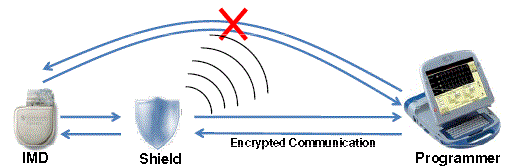
\includegraphics[width=0.7\textwidth]{resources/shield1.png}
    \caption{Schutz der Kommunikation zwischen Programmer und IMG durch das
    Shield \protect\cite{gollakota2011they}}
    \label{fig:shield1}
\end{figure}

\begin{figure}[htb]
    \centering
    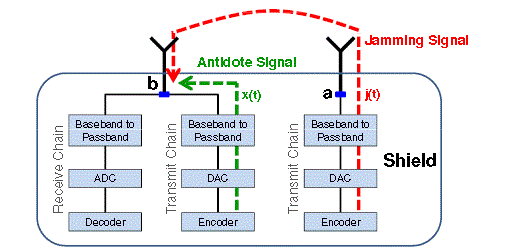
\includegraphics[width=0.7\textwidth]{resources/shield2.png}
    \caption{Kommunikationsdesign innerhalb des Shields \protect\cite{gollakota2011they}}
    \label{fig:shield2}
\end{figure}

\section{Fazit, Zusammenfassung und Ausblick}
Im medizinischen Bereich nehmen die Sicherheit und Privatsph�re von Patienten,
sowie die Zuverl�ssigkeit der Technik einen sehr hohen Stellenwert ein. Da
implantierbare medizintechnische Ger�te erst innerhalb des letzten Jahrzehnts
weite Verbreitung fanden, hat es einen gewissen Zeitraum gedauert bis in diesem
Bereich ernstzunehmende Anstrengungen unternommen wurden, die darauf
ausgerichtet waren einen hohen Sicherheitsstandard zu gew�hrleisten.

Herk�mmliche Sicherheitstechniken aus dem IT-Bereich k�nnen im Kontext von IMGs
nur bedingt angewandt werden, da die meisten implantierten Ger�te
batteriebetrieben sind und somit das Streben nach Energieeffizienz ein
konkurrierendes Ziel darstellt, wobei keines der beiden vernachl�ssigbar werden
darf. In Zukunft gilt es schrittweise Optimierungen vorzunehmen und effiziente
Methoden miteinander zu kombinieren um den Erreichungsgrad beider Ziele steigern
zu k�nnen.


\clearpage

 


\printindex

\pagestyle{empty}
\bibliography{bib/library}

\clearpage

%\include{biodata}

\end{document}
